\pagestyle{fancy}
\fancyhead[l]{\autorUO}
\fancyfoot[l]{\asignaturaAbbr}
\fancyfoot[r]{\fecha}

\section{\zorder} \label{sec:4}
En esta sección se estudia el rendimiento del esquema de acceso a memoria \zorder\ en cuanto al producto de matrices.
Para ello, se ha realizado dicha operación para los siguientes tamaños de matrices:
$\{2,\ 4,\ 8,\ 16,\ 32,\ 64,\ 128,\\ \ 256, \ 398,\ 512,\ 636,\ 774,\ 892,\ 1024,\ 1152,\ 1280,\ 1408,\ 1536\}$. 
Para cada tamaño de matriz, se ha probado con todos los tamaños de bloque posibles, incluyendo el tamaño de bloque $1$ y el del propio tamaño de la matriz. 
Cada producto se ha realizado un total de 32 veces y se ha medido el tiempo medio de ejecución. \\
Como los resultados para cada tamaño de matriz dependen del tamaño de bloque, las gráficas a mostrar son las resultantes de las ejecuciones 
de tamaños de matriz específicos, donde se pueden observar los tiempos de ejecución para cada tamaño de bloque. 
En la \autoref{fig:3} se muestran los resultados obtenidos para el tamaño de matriz $1024 \times 1024$.

\begin{figure}[h]
    \centering
    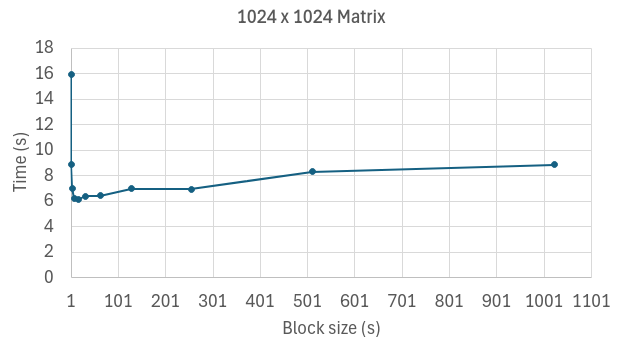
\includegraphics[width=0.5\textwidth]{img/3.png}
    \caption{Tiempos de ejecución de \zorder\ para el tamaño de matriz $1024 \times 1024$}
    \label{fig:3}
\end{figure}

\noindent{Se observa a simple vista una tendencia que se repite en todos los tamaños de matriz probados:}
\begin{itemize}
    \item El tamaño de bloque $1$ es el que más tiempo de ejecución requiere.
    \item Los tamaños de bloque relativamente pequeños ($4$, $8$, $16$ y $32$ en este caso) son los que mejores resultados ofrecen.
    \item A partir de cierto valor de tamaño de bloque, el tiempo de ejecución comienza a aumentar.
\end{itemize}
\vspace{0.25cm}
\noindent{Esta tendencia se repite de forma similar para todos los tamaños de matriz probados. Véase en la \autoref{fig:4} los 
resultados obtenidos para el tamaño de matriz $1280 \times 1280$ y en la \autoref{fig:5} los resultados obtenidos para el tamaño de matriz $1536 \times 1536$.}

\begin{figure}[h]
    \centering
    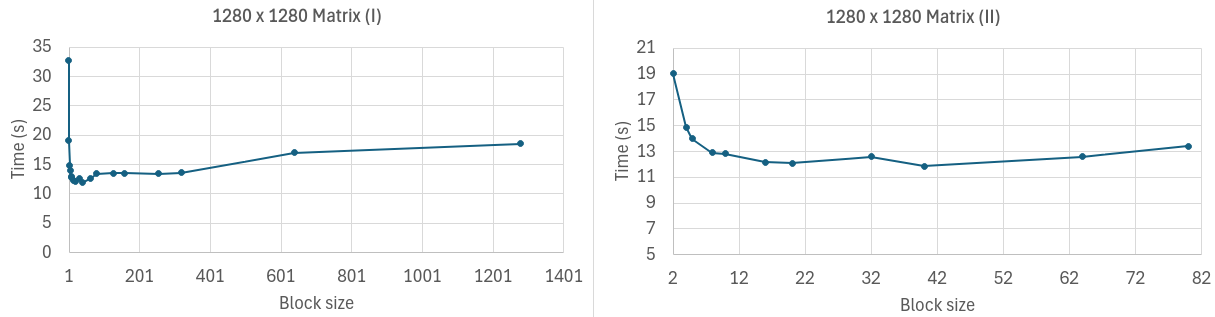
\includegraphics[width=0.85\textwidth]{img/4.png}
    \caption{Tiempos de ejecución de \zorder\ para el tamaño de matriz $1280 \times 1280$}
    \label{fig:4}
\end{figure}

\newpage

\begin{figure}[h]
    \centering
    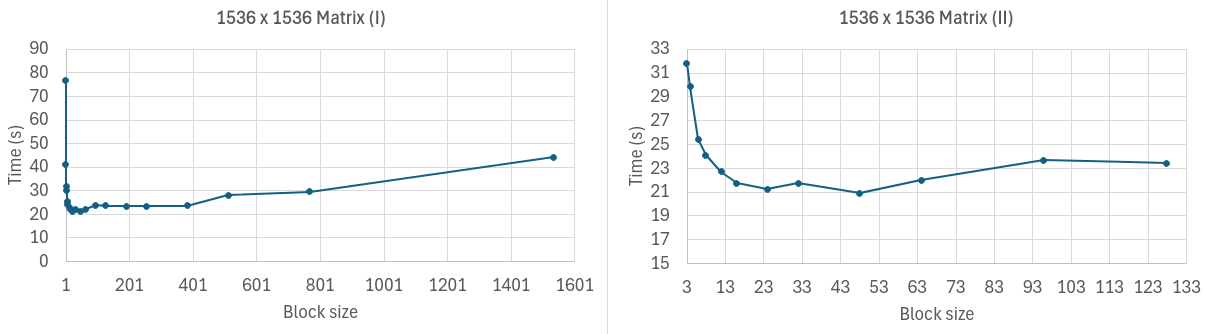
\includegraphics[width=0.85\textwidth]{img/5.png}
    \caption{Tiempos de ejecución de \zorder\ para el tamaño de matriz $1536 \times 1536$}
    \label{fig:5}
\end{figure}

Por lo tanto, se puede concluir que el uso de \zorder\ es muy eficiente si se utilizan tamaños de bloque óptimos, 
en concreto, tamaños de bloque relativamente pequeños (valores entre $8$ y $64$ válidos para el tamaño de matriz específico).
Sin embargo, el uso de tamaños de bloque demasiado pequeños o demasiado grandes puede resultar en un rendimiento muy deficiente.

Para terminar con este estudio, se analizará el rendimiento de \zorder\ respecto al de los esquemas de acceso a memoria \rowmajor\ y \colmajor.
Concretamente se comparará, para cada tamaño de matriz, el tiempo de ejecución de \rowmajor\ y \colmajor\ con el de \zorder\ 
utilizando el tamaño de bloque más óptimo en cada caso. Los resultados se muestran en la \autoref{tab:1}. Se han omitido los tamaños 
de matriz pequeños ya que no son representativos.

\renewcommand{\arraystretch}{1.25}
\begin{table}[h]
    \centering
    \begin{tabular}{|c|c|c|c|}
        \hline
        Matrix size & \rowmajor\ (s) & \colmajor\ (s) & \zorder\ (s) \\ \hline
        $[...]$ & $[...]$ & $[...]$ & $[...]$ \\ 
        $256 \times 256$ & $0.09026$ & $0.089583$ & $0.089992$ \\ 
        $398 \times 398$ & $0.394595$ & $0,388266$ & $\mathbf{0.375128}$ \\
        $512 \times 512$ & $0.946308$ & $0.902864$ & $\mathbf{0.747350}$ \\
        $636 \times 636$ & $1.784823$ & $1.702211$ & $\mathbf{1.447440}$ \\
        $774 \times 774$ & $3.397629$ & $3.167861$ & $\mathbf{2.548269}$ \\
        $892 \times 892$ & $5.104598$ & $4.827320$ & $\mathbf{4.665994}$ \\
        $1024 \times 1024$ & $8.473015$ & $7.278059$ & $\mathbf{6.071009}$ \\
        $1152 \times 1152$ & $12.413447$ & $10.524069$ & $\mathbf{8.527498}$ \\
        $1280 \times 1280$ & $17.331966$ & $14.561772$ & $\mathbf{11.818383}$ \\
        $1408 \times 1408$ & $27.91348$ & $22.76128$ & $\mathbf{15.968882}$ \\
        $1536 \times 1536$ & $42.912048$ & $32.64931$ & $\mathbf{20.887361}$ \\ \hline
    \end{tabular}
    \caption{Tiempos de ejecución de \rowmajor, \colmajor\ y mejor \zorder}
    \label{tab:1}
\end{table}
\renewcommand{\arraystretch}{1.0}

A simple vista se observa que el rendimiento de \zorder\ es muy similar en tamaños de matrices medianos y mucho mejor en 
tamaños de matrices grandes. Concretamente, su rendimiento mejora respecto a \rowmajor\ y \colmajor\ a medida que el tamaño de matriz aumenta.